%\documentclass[a4paper]{article}
%
%% subfile handling packages
%\usepackage{subfiles}
%\newcommand{\onlyinsubfile}[1]{#1}
%\newcommand{\notinsubfile}[1]{}
%
%% document packages
%\usepackage[top=1in, bottom=1.25in, left=1.25in, right=1.25in]{geometry}
%\usepackage{amsmath}
%\usepackage{multicol}
%\usepackage{caption}
%\usepackage{subcaption}
%\usepackage{graphicx}
%\usepackage{multirow}
%\usepackage{tabulary}
%\usepackage{hhline}
%\usepackage{indentfirst}
%\RequirePackage{ltxcmds}[2010/12/07]
%\graphicspath{{../../images/}}
%%\graphicspath
%\usepackage{float}
%\usepackage{amsfonts}
%\usepackage{hyperref}
%\usepackage{footnote}
%\makesavenoteenv{tabular}
%\usepackage{braket}
%%opening
%\title{Safety study}
%\author{}
%\date{}
%
%
%\begin{document}
%\maketitle
\clearpage
\section{Continuos Variable Quantum Transmission System}\label{sec:intro}

In this section a continuous varible quantum transmission system is analyzed.
The results here presented follow closely the~\cite{namiki2003security}.
In~\cite{namiki2003security}, the security of a continuous variable quantum key distribution (CV-QKD) system is studied theoretically, here we complete that theoretical study with simulations results.

\begin{figure}[h]
\centering
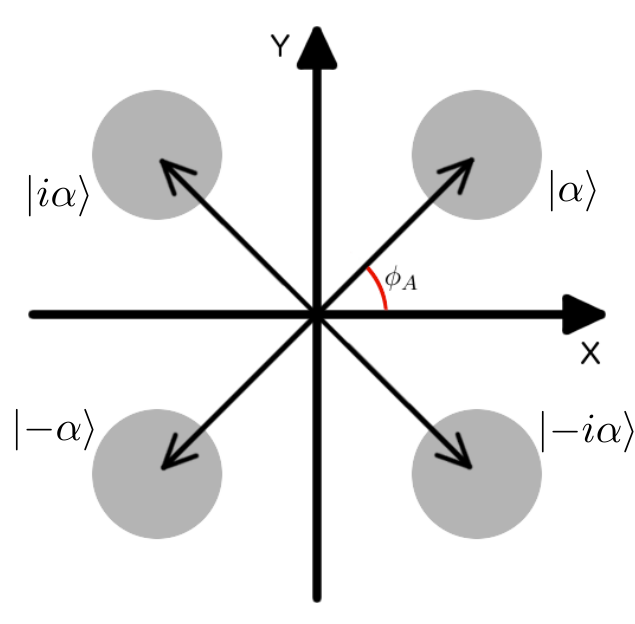
\includegraphics[width=.5\linewidth]{./sdf/cv_system/figures/constellation.png}
\caption{State constellation}
\label{fig:const}
\end{figure}

The state constellation used in the system is presented in Figure~\ref{fig:const}.
The emitter (usually named Alice) is going to use two basis, the $45º$ base and the $-45º$ base.
In the $45º$ base, Alice sends one of two values, $1$ and $-1$, which correspond to the states $\ket{\alpha}$ and $\ket{-\alpha}$.
In the $-45º$ base, Alice can also send one of two values, $1$ and $-1$, which correspond to the states $\ket{-i\alpha}$ and $\ket{i\alpha}$.
At the end Alice is going to send one of the four states $\ket{\alpha}$, $\ket{-\alpha}$, $\ket{-i\alpha}$, and $\ket{i\alpha}$, with equal probability.

Because we don't know $\grave{a}$ prior which state is going be transmitted, neither which basis is going to be used, and to incorporate our ``ignorance"\, in the system description, we can work with the density operator. The density operator is a proper tool to describe ``statistical mixtures". A ``statistical mixtures" is one state, from a possible set, but we don't know which state it is. There is no state superposition.

Since all states have the same probability of occurring, the state density operator is given by:

\begin{equation}\label{eq:statedensity}
\hat{\rho}=\frac{1}{4}\left(\ket{\alpha}\bra{\alpha}+\ket{-\alpha}\bra{-\alpha}+\ket{i\alpha}\bra{i\alpha}+\ket{-i\alpha}\bra{-i\alpha}\right).
\end{equation}

The probability to detect at the receiver the state $\ket{\alpha}$ is given by
\begin{equation}\label{eq:statedensity}
P(\alpha)=\bra{\alpha}\hat{\rho}\ket{\alpha}=\frac{1}{4}.
\end{equation}


Note that the density operator is equivalent to the wave function in terms of the system description.

From the receiver perspective, i.e. from the Bob perspective, and after knowing the base used by Alice.
The density operator can be reduce to,

\begin{align}
\hat{\rho}_1&=\frac{1}{2}\left(\ket{\alpha}\bra{\alpha}+\ket{-\alpha}\bra{-\alpha}\right),\label{eq:statedensity1} \\
\hat{\rho}_2&=\frac{1}{2}\left(\ket{i\alpha}\bra{i\alpha}+\ket{-i\alpha}\bra{-i\alpha}\right).\label{eq:statedensity2}
\end{align}

where $1$ corresponds to the $45º$ base and $-1$ corresponds to $-45º$.

\subsubsection*{Single Base Homodyne Detection}


The probability of obtaining a quadrature $\hat{X}_\phi=\hat{X}_1\cos\phi+\hat{X}_2\sin\phi$ when measuring the coherent state $\ket{\alpha}$ is given by the following gaussian distribution:

\begin{equation}
\left|\braket{X_\phi|\alpha}\right|^2=\sqrt{\frac{2}{\pi}}e^{-2(X_\phi-\alpha\cos\phi)^2},
\end{equation}

We can define the "correct" and "wrong" basis measurement probability density, respectively, as:

\begin{equation}\label{eq:probdensity}
\bra{X_i}\hat{\rho}_j\ket{X_i}=
\begin{cases}
\frac{1}{\sqrt{2\pi}}\left(e^{-2(X_i-\alpha)^2}+e^{-2(X_i+\alpha)}\right), & i=j\\
\sqrt{\frac{2}{\pi}}e^{-2X_i^2}, &i\neq j
\end{cases}.
\end{equation}

The post selection efficiency (PSE) can be defined as the probability of a measurement in the correct basis yields a result that satisfies the limit value $X_0$:

\begin{equation}\label{eq:postselecteff}
\begin{aligned}
P(X_0,\alpha)&=\int^{-X_0}_{-\infty}\bra{X_1}\hat{\rho}_1\ket{X_1}dX_1+\int^{\infty}_{X_0}\bra{X_1}\hat{\rho}_1\ket{X_1}dX_1\\
&=\frac{1}{2}\left[\text{erfc}(\sqrt{2}(X_0+\alpha))+\text{erfc}(\sqrt{2}(X_0-\alpha))\right].
\end{aligned}
\end{equation}

The bit error rate (BER) is the normalized probability of, after choosing the correct basis, obtaining the wrong bit value:

\begin{equation}\label{eq:biterrorratio}
Q(X_0,\alpha)=\frac{1}{P(X_0,\alpha)}\int_{-\infty}^{-X_0}\left|\braket{X_i|\alpha}\right|dX_i=\frac{\text{erfc}\left(\sqrt{2}(X_0+\alpha)\right)}{2P(X_0,n)}
\end{equation}

\begin{figure}[h]
\centering
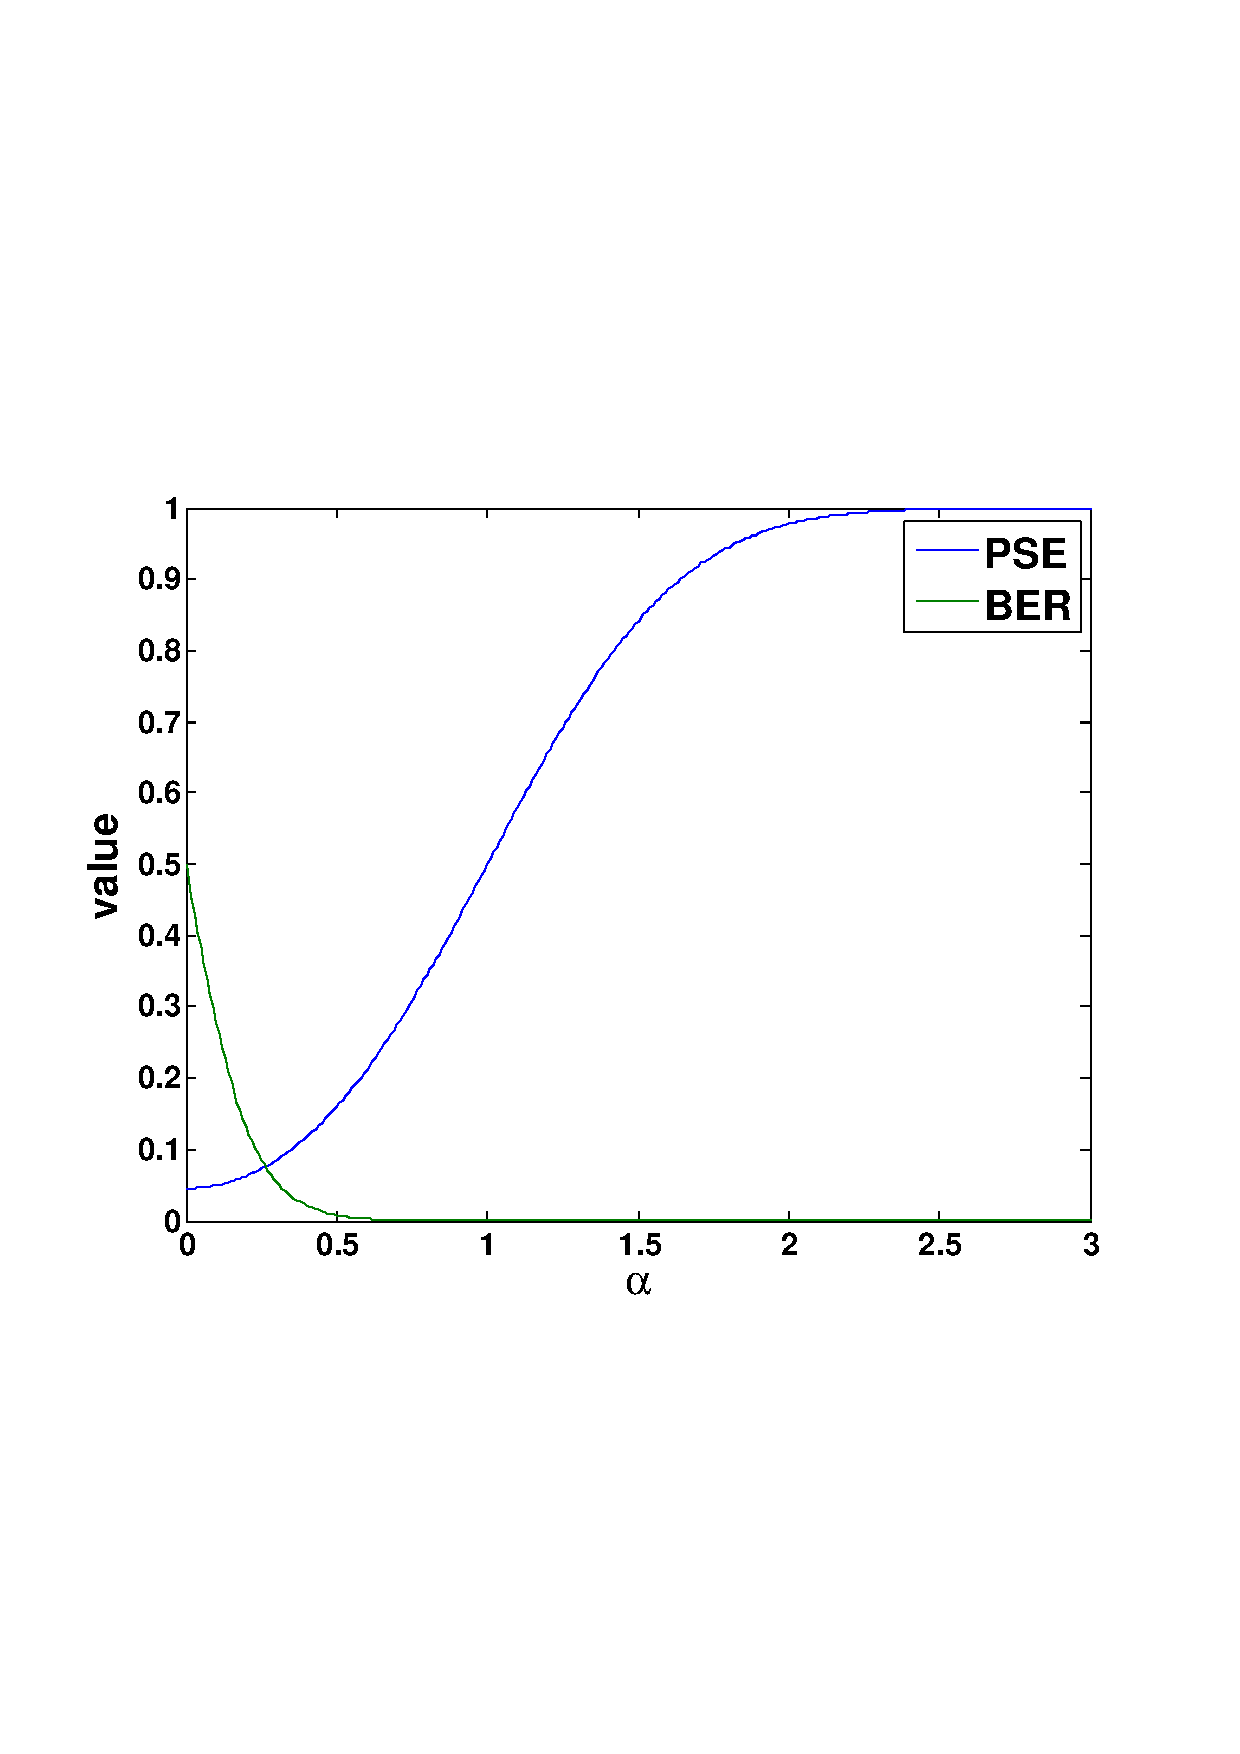
\includegraphics[width=\linewidth, trim= 0mm 60mm 0mm 70mm]{./sdf/cv_system/figures/singlehomodyne.pdf}
\caption{BER and PSE in function of $\alpha$ for the single homodyne setup. $X_0=1$ was used}
\label{fig:ber}
\end{figure}



\subsubsection*{Double Homodyne setup}

In our proposed double homodyne protocol both quadratures are measured simultaneously, as such the concept of correct and wrong basis measurements has no value. Our protocol also makes use of a locally generated Local Oscillator (LO), obtained from a different laser than the one used to generate the signal, thus we have to take into account the phase drift between both lasers. High intensity reference pulses are sent periodically to allow for an estimation of the phase drift. The double homodyne setup requires the signal to be divided into the two utilized detectors, so each measurement is made on a coherent state with half the amplitude of the incoming signal $\alpha\rightarrow\frac{\alpha}{\sqrt{2}}$
\par
For each incoming pulse we measure quadratures $X_\phi$ and $Y_\phi$. $\phi$ has contributions from both the encoded angle, $\theta$, and the phase difference between lasers, $\epsilon$, we assume $\phi=\theta+\epsilon$. On the reference pulses no phase is encoded, that is $\theta=0$, thus $\epsilon$ can be estimated. Assuming $\epsilon$ doesn't change between a reference pulse and the following signal pulse, the measured quadratures can be cast into the originally sent quadratures $X_\theta$ and $Y_\theta$ via:
\begin{equation}
\begin{aligned}
X_\theta&=X_\phi\cos\epsilon-Y_\phi\sin\epsilon\\
Y_\theta&=X_\phi\sin\epsilon+Y_\phi\sin\epsilon
\end{aligned}
\end{equation}
Assuming an announcement of the coding basis, the density operators~\eqref{eq:statedensity1} and~\eqref{eq:statedensity2} still apply. We can now define the probability density of obtaining results $X_\theta$ and $Y_\theta$, assuming a state in the $X_1$ base was sent, as:
\begin{align}
\braket{X_\theta|\hat{\rho}_1|X_\theta}&= \frac{\sqrt{\frac{2}{\pi}}}{4}\left(e^{-2\left(x_\theta-\frac{\alpha}{\sqrt{2}}\cos\theta\right)^2}+e^{-2\left(x_\theta+\frac{\alpha}{\sqrt{2}}\cos\theta\right)^2}\right),\\
\braket{Y_\theta|\hat{\rho_1}|Y_\theta}&= \frac{\sqrt{\frac{2}{\pi}}}{4}\left(e^{-2\left(y_\theta-\frac{\alpha}{\sqrt{2}}\sin\theta\right)^2}+e^{-2\left(y_\theta+\frac{\alpha}{\sqrt{2}}\sin\theta\right)^2}\right).
\end{align}
\par
Now each state needs to satisfy two limit values, $X_0$ and $Y_0$, to be accepted. Thus, the PSE is now defined as:
\begin{equation}
\begin{aligned}
P_{DH}(X_0,Y_0,\alpha)&=\int^{-X_0}_{-\infty}\braket{X_\theta|\hat{\rho}_1|X_\theta}dx_\theta\int^{-Y_0}_{-\infty}\braket{Y_\theta|\hat{\rho}_1|Y_\theta}dy_\theta+\\
&\int_{X_0}^{\infty}\braket{X_\theta|\hat{\rho}_1|X_\theta}dx_\theta\int_{Y_0}^{\infty}\braket{Y_\theta|\hat{\rho}_1|Y_\theta}dy_\theta\\
&=\frac{1}{4}\left\lbrace\text{erfc}\left[\sqrt{2}\left(X_0-\frac{\alpha}{\sqrt{2}}\cos\theta\right)\right]+\text{erfc}\left[\sqrt{2}\left(X_0+\frac{\alpha}{\sqrt{2}}\cos\theta\right)\right]\right\rbrace\\
&\left\lbrace\text{erfc}\left[\sqrt{2}\left(Y_0-\frac{\alpha}{\sqrt{2}}\sin\theta\right)\right]+\text{erfc}\left[\sqrt{2}\left(Y_0+\frac{\alpha}{\sqrt{2}}\sin\theta\right)\right]\right\rbrace,
\end{aligned}
\end{equation}
The DH subscript denotes Double Homodyne. In a somewhat similar manner, the BER is now defined as:
\begin{equation}\label{eq:adaptedBER}
\begin{aligned}
Q_{DH}(X_0,Y_0,\alpha)&=\frac{1}{P_{DH}}\left(\int^{-X_0}_{-\infty}\left|\braket{X_\theta|\frac{\alpha}{\sqrt{2}}}\right|^2dx_\theta\int^{-Y_0}_{-\infty}\left|\braket{Y_\theta|\frac{\alpha}{\sqrt{2}}}\right|^2dy_\theta+\right.\\
&\left.\int_{X_0}^{\infty}\left|\braket{X_\theta|-\frac{\alpha}{\sqrt{2}}}\right|^2dx_\theta\int_{Y_0}^{\infty}\left|\braket{Y_\theta|-\frac{\alpha}{\sqrt{2}}}\right|^2dy_\theta\right)\\
&=\frac{1}{2P_{DH}}\text{erfc}\left[\sqrt{2}\left(X_0+\frac{\alpha}{\sqrt{2}}\cos\theta\right)\right]\text{erfc}\left[\sqrt{2}\left(Y_0+\frac{\alpha}{\sqrt{2}}sin\theta\right)\right],
\end{aligned}
\end{equation}
note that, in this definition for BER, only values $\theta\in\left[0,\frac{\pi}{2}\right]$ make sense (the sent state was $\alpha$).

\begin{figure}[h]
\centering
\begin{subfigure}{.48\linewidth}
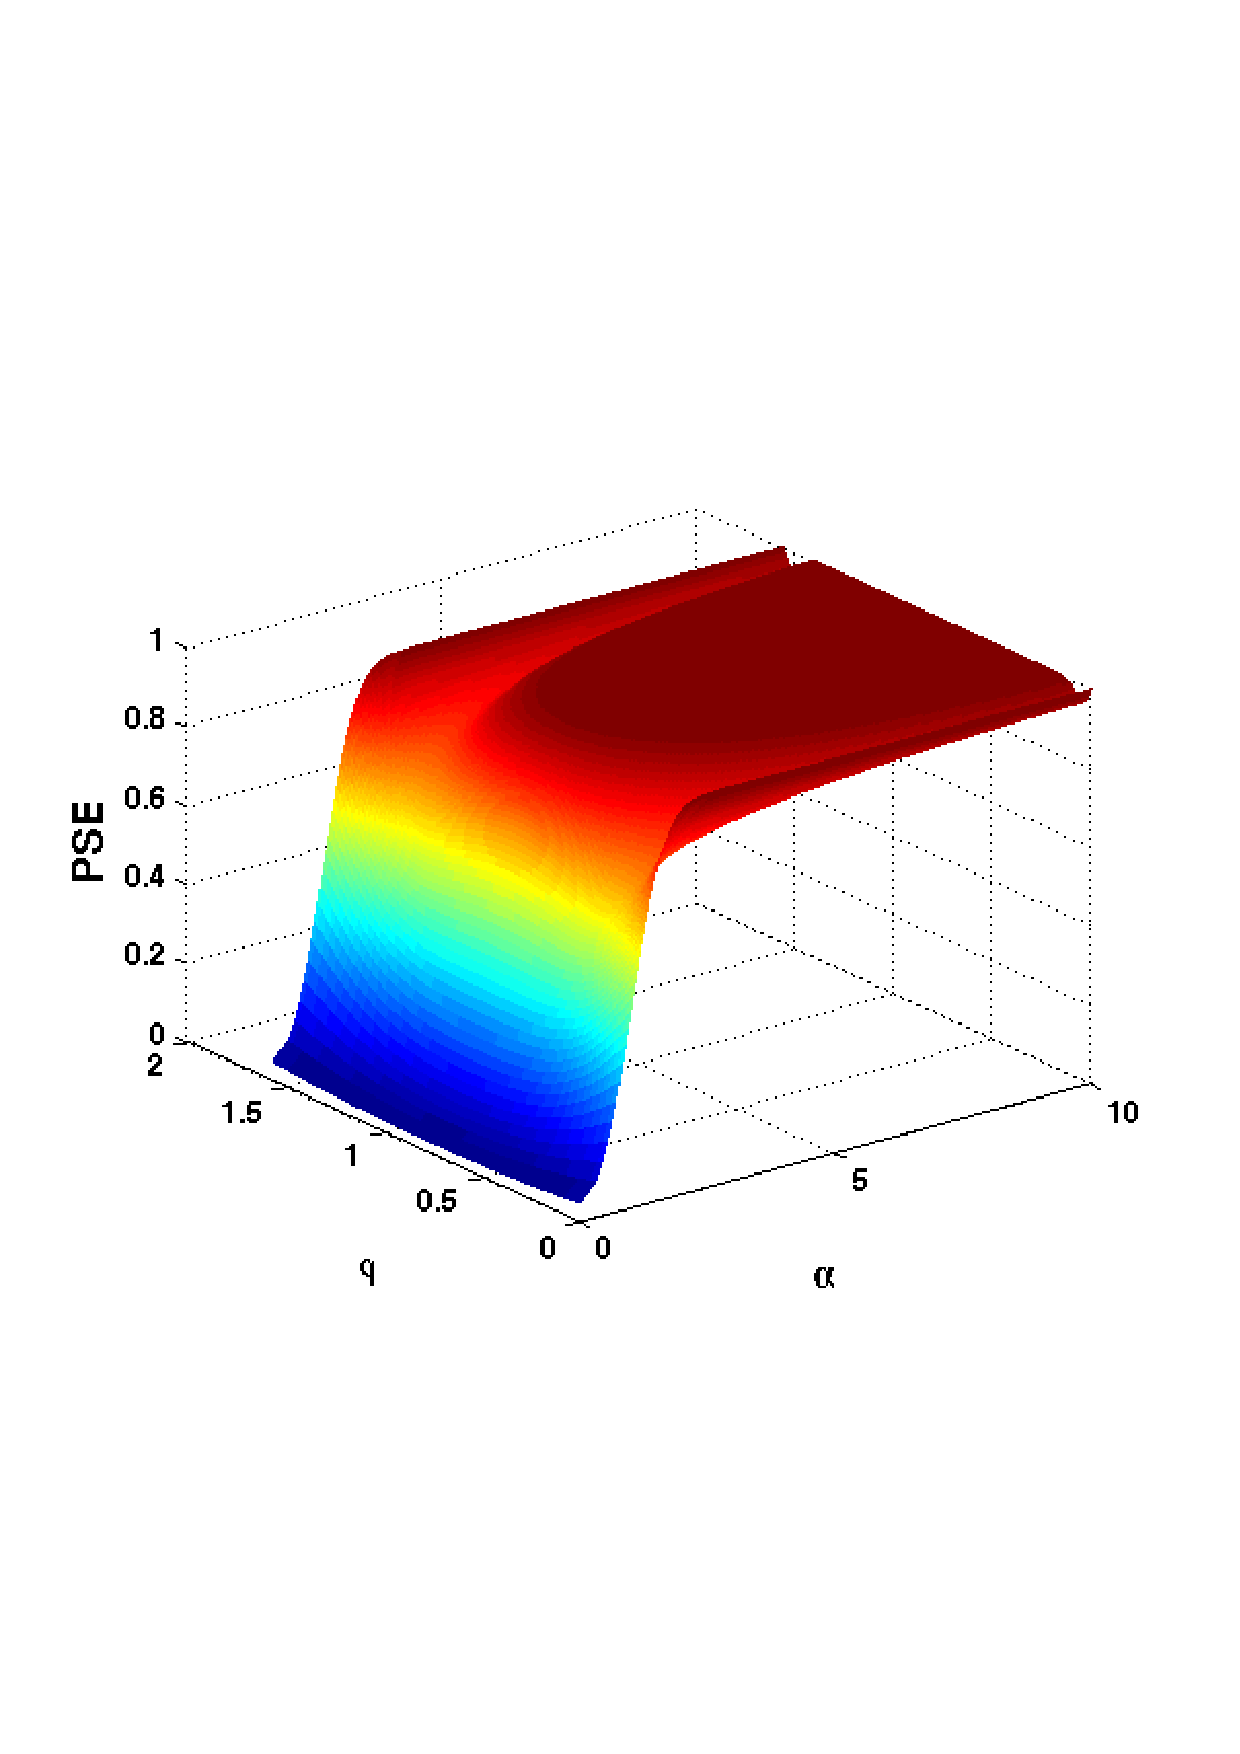
\includegraphics[width=\linewidth, trim= 0mm 60mm 0mm 70mm]{doublehomodynePSE.pdf}
\caption{PSE in function of $\alpha$ and $\theta$ for the double homodyne setup. $X_0=1$ was used}
\end{subfigure}
~
\begin{subfigure}{.48\linewidth}
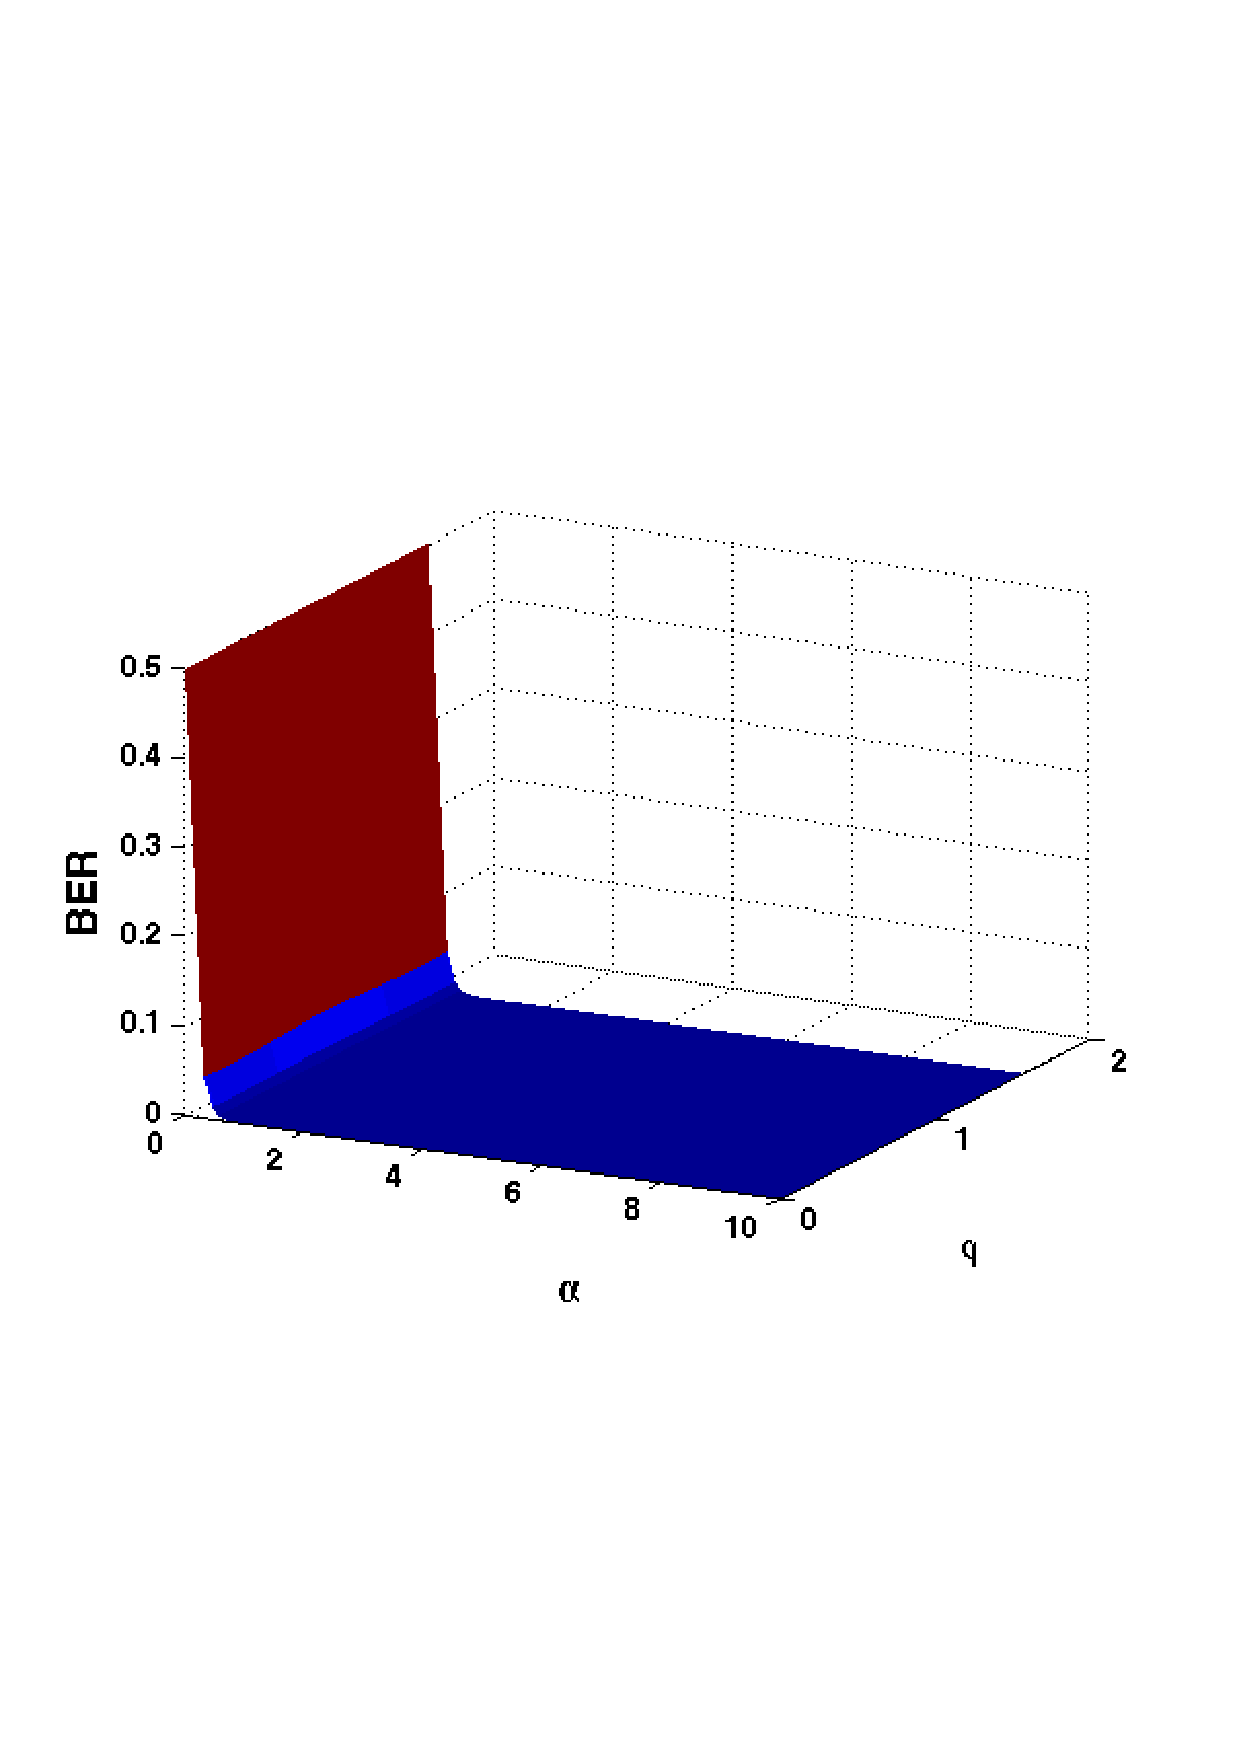
\includegraphics[width=\linewidth, trim= 0mm 60mm 0mm 70mm]{doublehomodyneBER.pdf}
\caption{BER in function of $\alpha$ and $\theta$ for the double homodyne setup. $X_0=1$ was used}
\end{subfigure}
\caption{Theoretical results for double homodyne setup.}
\end{figure}

\subsection*{Functional Description}

Simplified diagrams of the systems being simulated are presented in Figures~\ref{fig:singleH}. and~\ref{fig:doubleH}. Two optical signals are generated, one with a constant power level of 10~dBm and the other with power in multiples of the power corresponding to a single photon per sampling time (6.4078e$\times10^{-13}$~W for a sampling time of 200~ns). The two signals are mixed, with a Balanced Beam Splitter in the single homodyne case and with a 90$^\text{o}$ Optical Hybrid in the double homodyne one, and are subsequently evaluated with recourse to Homodyne Receivers.

\begin{figure}[h]
\centering
\begin{subfigure}{\linewidth}
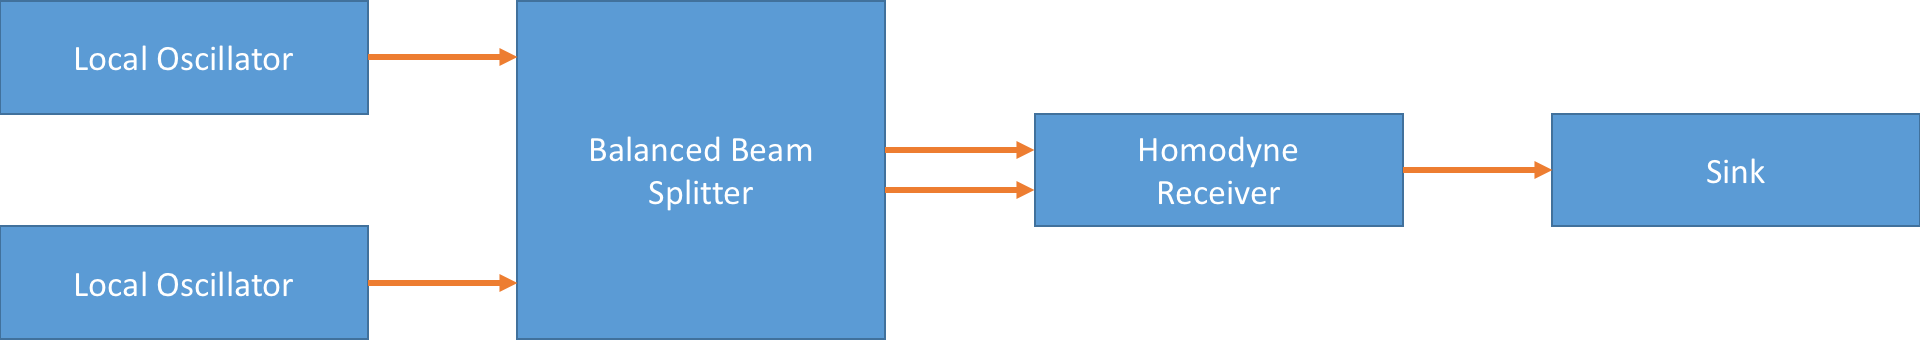
\includegraphics[width=\linewidth]{singlehomodyneSimuBlock.png}
\caption{Single homodyne simulation block diagram.}
\label{fig:singleH}
\end{subfigure}
\\
~
\\
\begin{subfigure}{\linewidth}
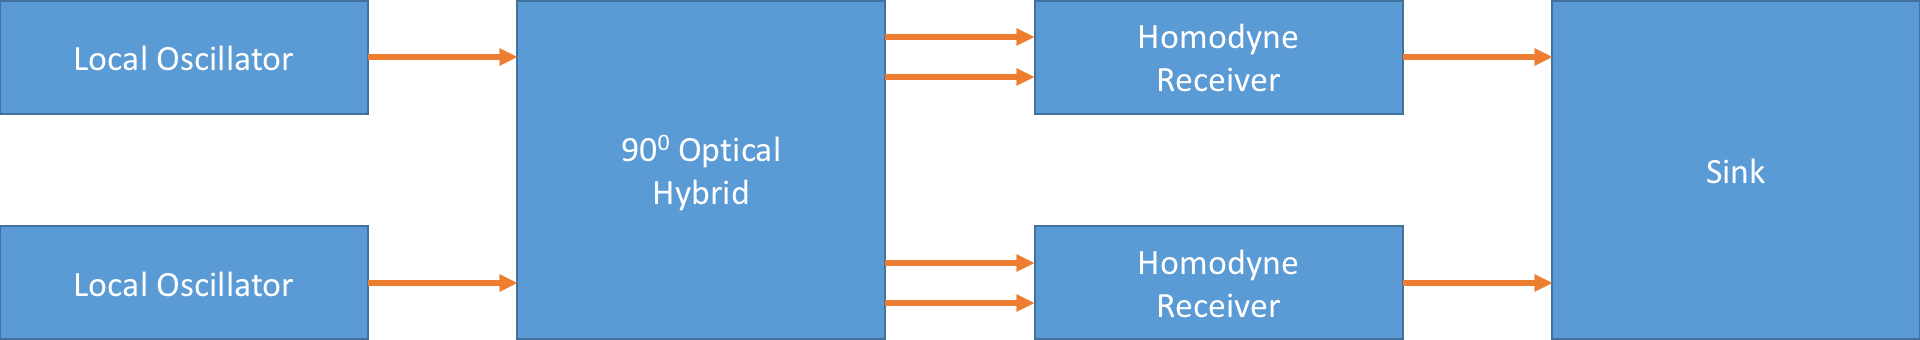
\includegraphics[width=\linewidth]{doublehomodyneSimuBlock.png}
\caption{Double homodyne simulation block diagram.}
\label{fig:doubleH}
\end{subfigure}
\caption{Block diagrams of both simulation results presented in this report.}
\end{figure}

\begin{table}[H]
\centering
\begin{tabular}{c|c}
System Blocks          & netxpto Blocks       \\ \hline
Local Oscillator       & LocalOscillator      \\
Homodyne Receiver      & I\_HomodyneReceiver   \\
Balanced Beam Splitter & BalancedBeamSplitter \\
90$^\text{o}$ Optical Hybrid     & OpticalHybrid
\end{tabular}
\end{table}

\pagebreak
\subsection*{Required files}\label{Required files}

Header Files
\begin{table}[H]
\centering
\begin{tabulary}{1.0\textwidth}{|L|L|}
\hline
\textbf{File}              & \textbf{Description} 				            \\ \hline
netxpto.h                  & Generic purpose simulator definitions.	        \\ \hline
local\_oscillator.h        & Generates continuous coherent signal.            \\ \hline
balanced\_beam\_splitter.h & Mixes the two input signals into two outputs.    \\ \hline
optical\_hybrid.h          & Mixes the two input signals into four outputs.   \\ \hline
homodyne\_reciever.h       & Performs coherent detection on the input signal. \\ \hline
sink.h                     & Closes any unused signals.                       \\ \hline
\end{tabulary}
\end{table}
%
Source Files
\begin{table}[H]
\centering
\begin{tabulary}{1.0\textwidth}{|L|L|}
\hline
\textbf{File}                & \textbf{Description} 					          \\ \hline
netxpto.cpp                  & Generic purpose simulator definitions.	          \\ \hline
local\_oscillator.cpp        & Generates continuous coherent signal.            \\ \hline
balanced\_beam\_splitter.cpp & Mixes the two input signals into two outputs.    \\ \hline
optical\_hybrid.cpp          & Mixes the two input signals into four outputs.   \\ \hline
homodyne\_reciever.cpp       & Performs coherent detection on the input signal. \\ \hline
sink.cpp                     & Closes any unused signals.                       \\ \hline
\end{tabulary}
\end{table}


\subsection*{System Input Parameters}

This system takes into account the following input parameters:
\begin{table}[H]
\centering
\begin{tabulary}{1.0\textwidth}{|C|C|}
\hline
\textbf{System Parameters} & \textbf{Description}                                                                   \\ \hline
numberOfBitsGenerated      & Gives the number of bits to be simulated                                               \\ \hline
bitPeriod                  & Sets the time between adjacent bits                                                    \\ \hline
samplesPerSymbol           & Establishes the number of samples each bit in the string is given                      \\ \hline
localOscillatorPower\_dBm1 & Sets the optical power, in units of dBm, at the reference output	                      \\ \hline
localOscillatorPower2      & Sets the optical power, in units of W, of the signal                                   \\ \hline
localOscillatorPhase1      & Sets the initial phase of the local oscillator used for reference                      \\ \hline
localOscillatorPhase2      & Sets the initial phase of the local oscillator used for signal                         \\ \hline
transferMatrix             & Sets the transfer matrix of the beam splitter used in the homodyne detector            \\ \hline
responsivity               & Sets the responsivity of the photodiodes used in the homodyne detector                 \\ \hline
amplification              & Sets the amplification of the trans-impedance amplifier used in the homodyne detector  \\ \hline
electricalNoiseAmplitude   & Sets the amplitude of the gaussian thermal noise added in the homodyne detector        \\ \hline
shotNoise                  & Chooses if quantum shot noise is used in the simulation                                \\ \hline
\end{tabulary}
\end{table}		

\subsection*{Inputs}

This system takes no inputs.
%
\subsection*{Outputs}

The single homodyne system outputs the following objects:
\begin{itemize}
\item Signals:
\begin{itemize}
\item Local Oscillator Optical Reference; (S$_{1}$)
\item Local Oscillator Optical Signal; (S$_{2}$)
\item Beam Splitter Outputs; (S$_{3}$, S$_{4}$)
\item Homodyne Detector Electrical Output; (S$_{5}$)
\end{itemize}
\end{itemize}
\par
The double homodyne system outputs the following objects:
\begin{itemize}
\item Signals:
\begin{itemize}
\item Local Oscillator Optical Reference; (S$_{1}$)
\item Local Oscillator Optical Signal; (S$_{2}$)
\item 90$^\text{o}$ Optical Hybrid Outputs; (S$_{3}$, S$_{4}$, S$_{5}$, S$_{6}$)
\item Homodyne Detector Electrical Output; (S$_{7}$)
\end{itemize}
\end{itemize}		

\subsection*{Simulation Results}
\subsubsection*{Single homodyne results}\label{subsec:SHresults}

The numerical results presented in Figure~\ref{fig:directber} were obtained with the simulation described by the block diagram in Figure~\ref{fig:singleH}. Theoretical results are a direct trace of~\eqref{eq:biterrorratio}. One can see that the numerical results adhere quite well to the expected curve.

\begin{figure}[h]
\centering
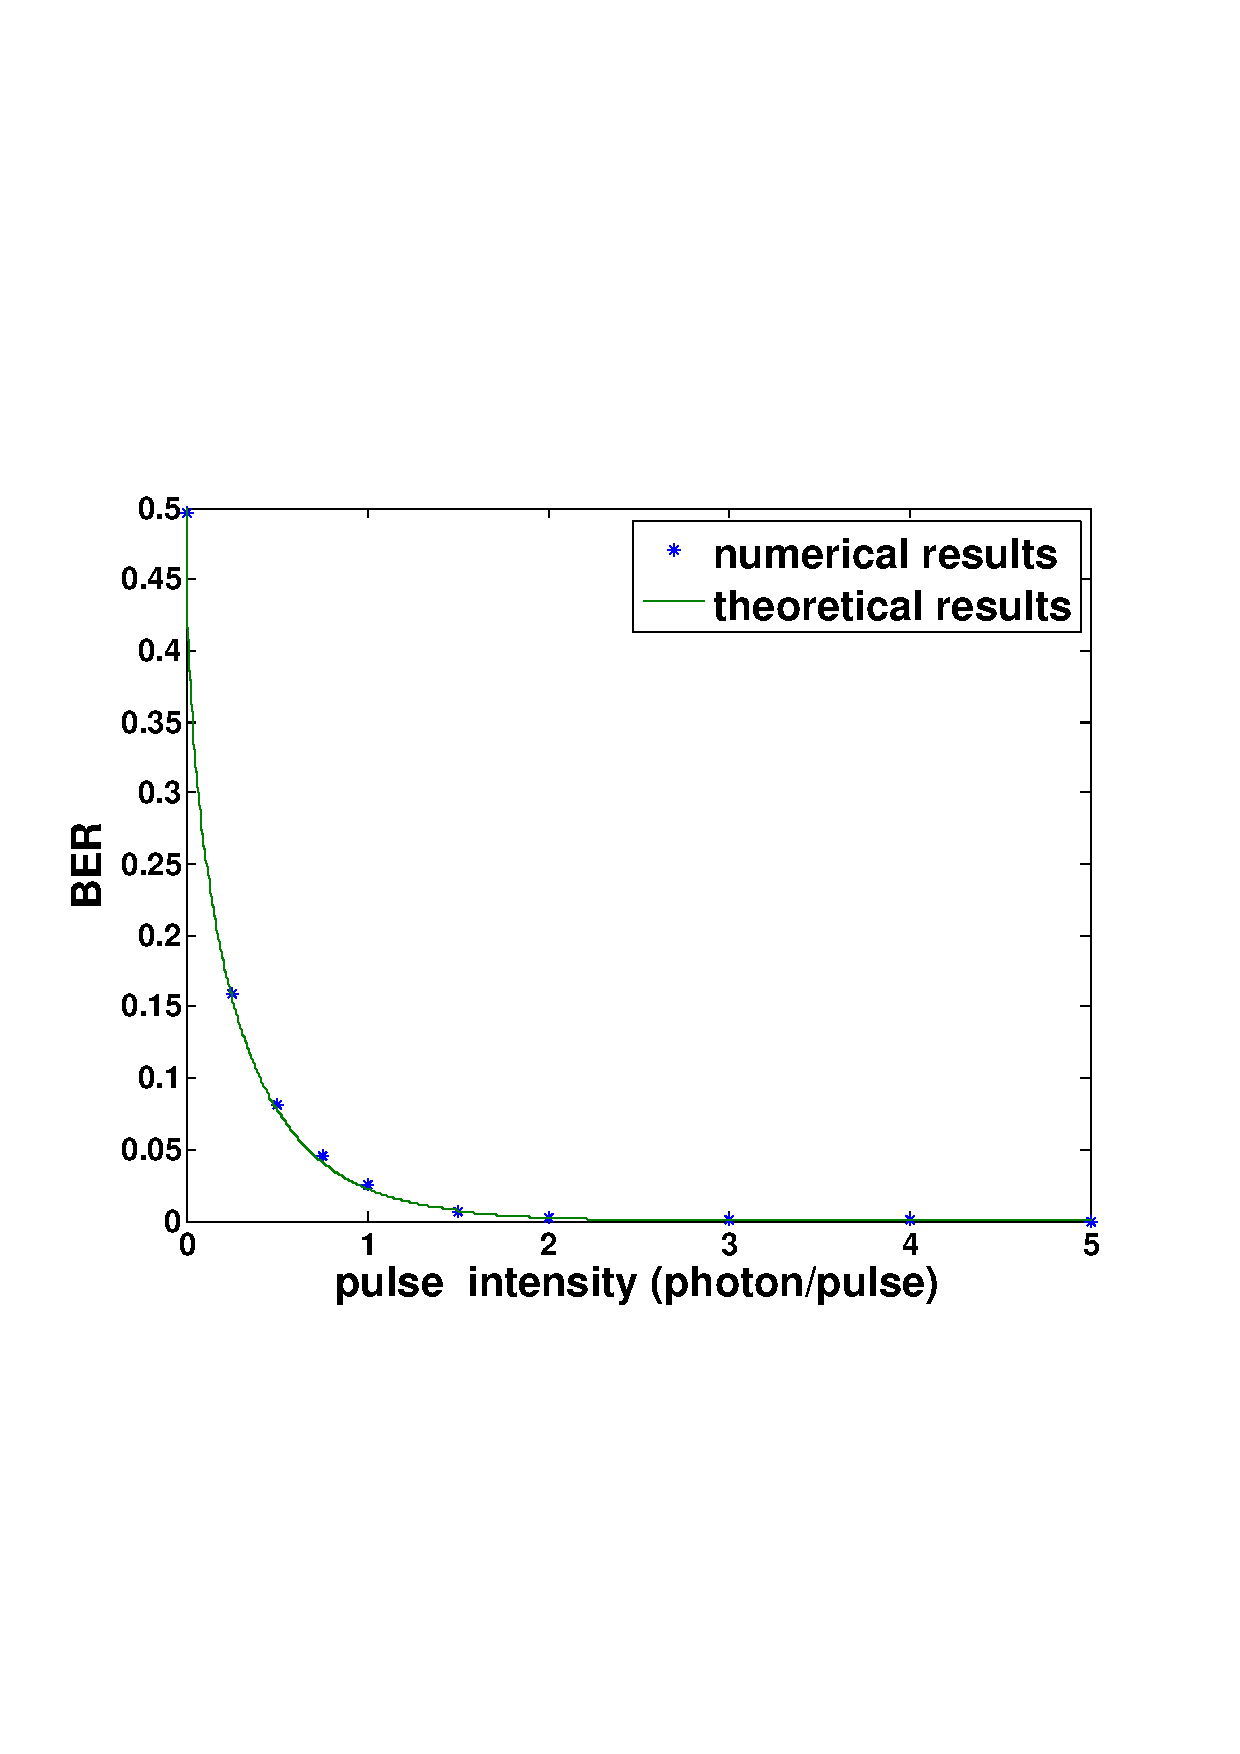
\includegraphics[width=\linewidth, trim= 0mm 60mm 0mm 70mm]{directBER.pdf}
\caption{BER in function of $\alpha$ for the single homodyne setup. $X_0=0$ was used}
\label{fig:directber}
\end{figure}

\subsubsection*{Double homodyne results}\label{subsec:DHresults}

The numerical results presented in Figure~\ref{fig:adaptedber} were obtained with the simulation described by the block diagram in Figure~\ref{fig:doubleH}. Theoretical results are a direct trace of~\eqref{eq:adaptedBER} with $\theta=\frac{\pi}{4}$. One can see that the numerical results adhere quite well to the expected curve.

\begin{figure}[h]
\centering
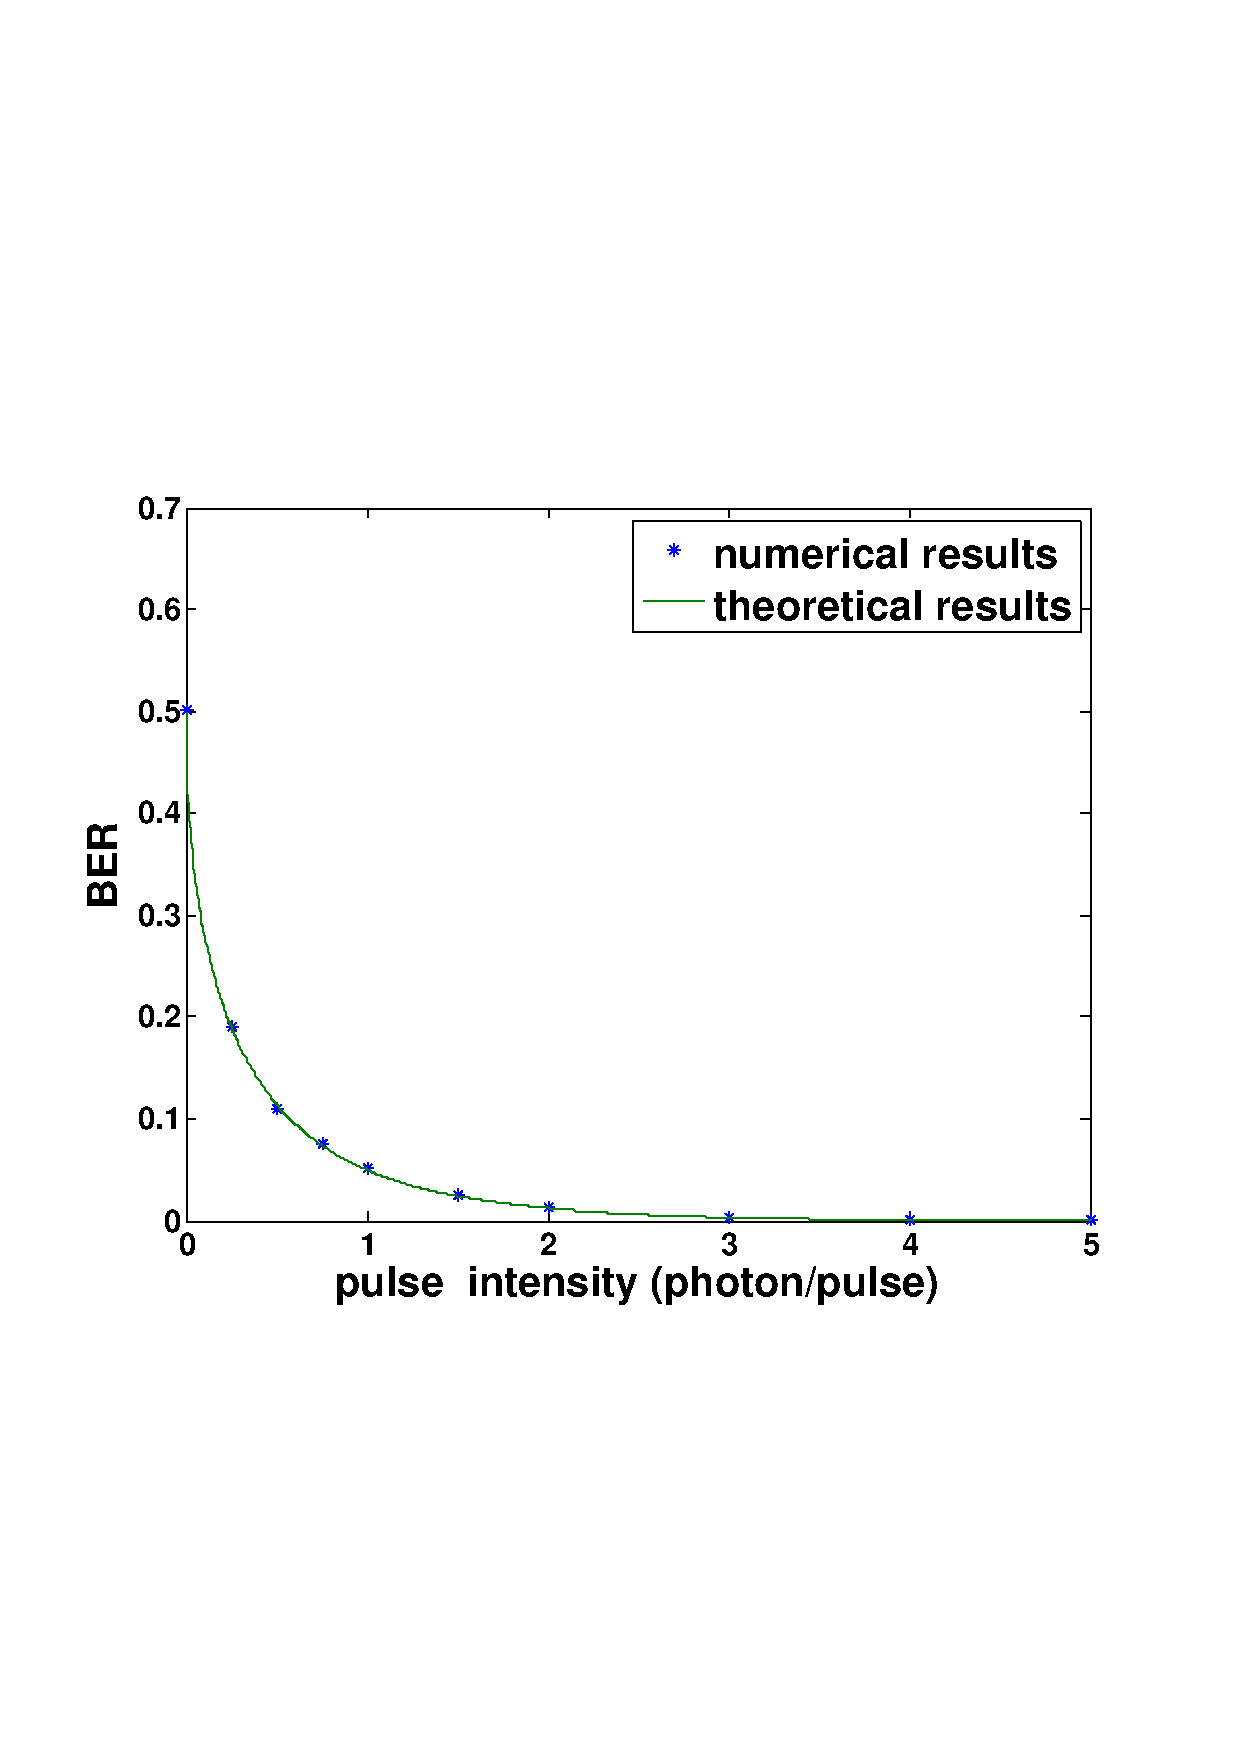
\includegraphics[width=\linewidth, trim= 0mm 60mm 0mm 70mm]{adaptedBER.pdf}
\caption{BER in function of $\alpha$ for the double homodyne setup. $X_0=0$ was used}
\label{fig:adaptedber}
\end{figure}

%\section{Block Description}
%
%\subsection{Homodyne Receiver}
%\subfile{./lib/i_homodyne_receiver}
%
%\subsection{Local Oscillator}
%\subfile{./lib/localoscillator}
%
%\subsection{Beam Splitter}
%\subfile{./lib/beamsplitter}
%
%\subsection{90$^\text{o}$ Optical Hybrid}
%
%\subsection{Photodiode}
%\subfile{./lib/photodiode}
%
%\subsection{Amplifier}
%\subfile{./lib/ideal_amplifier}
%
%\subsection{Electrical Filter}
%\subfile{./lib/pulse_shaper}

\subsection*{Known Problems}
\begin{enumerate}
    \item Homodyne Super-Block not functioning
    \item 90$^\text{o}$ Optical Hybrid PDF needs to be written
\end{enumerate}


\bibliographystyle{unsrt}
\bibliography{bibliography}
%\end{document} 